%%%%%%%%%%%%%%%%%%%%%%%%%%%%%%%%%%%%%%%%%%%%%%%%%%%%%%%%%%%%%%%%%%%%%%
%%  Copyright by Wenliang Du.                                       %%
%%  This work is licensed under the Creative Commons                %%
%%  Attribution-NonCommercial-ShareAlike 4.0 International License. %%
%%  To view a copy of this license, visit                           %%
%%  http://creativecommons.org/licenses/by-nc-sa/4.0/.              %%
%%%%%%%%%%%%%%%%%%%%%%%%%%%%%%%%%%%%%%%%%%%%%%%%%%%%%%%%%%%%%%%%%%%%%%

\newcommand{\commonfolder}{../../common-files}

\documentclass[11pt]{article}

\usepackage[most]{tcolorbox}
\usepackage{times}
\usepackage{epsf}
\usepackage{epsfig}
\usepackage{amsmath, alltt, amssymb, xspace}
\usepackage{wrapfig}
\usepackage{fancyhdr}
\usepackage{url}
\usepackage{verbatim}
\usepackage{fancyvrb}
\usepackage{adjustbox}
\usepackage{listings}
\usepackage{color}
\usepackage{subfigure}
\usepackage{cite}
\usepackage{sidecap}
\usepackage{pifont}
\usepackage{mdframed}
\usepackage{textcomp}
\usepackage{enumitem}
\usepackage{hyperref}


% Horizontal alignment
\topmargin      -0.50in  % distance to headers
\oddsidemargin  0.0in
\evensidemargin 0.0in
\textwidth      6.5in
\textheight     8.9in 

\newcommand{\todo}[1]{
\vspace{0.1in}
\fbox{\parbox{6in}{TODO: #1}}
\vspace{0.1in}
}


\newcommand{\unix}{{\tt Unix}\xspace}
\newcommand{\linux}{{\tt Linux}\xspace}
\newcommand{\minix}{{\tt Minix}\xspace}
\newcommand{\ubuntu}{{\tt Ubuntu}\xspace}
\newcommand{\setuid}{{\tt Set-UID}\xspace}
\newcommand{\openssl} {\texttt{openssl}}


\pagestyle{fancy}
\lhead{\bfseries SEED Labs}
\chead{}
\rhead{\small \thepage}
\lfoot{}
\cfoot{}
\rfoot{}


\definecolor{dkgreen}{rgb}{0,0.6,0}
\definecolor{gray}{rgb}{0.5,0.5,0.5}
\definecolor{mauve}{rgb}{0.58,0,0.82}
\definecolor{lightgray}{gray}{0.90}


\lstset{%
  frame=none,
  language=,
  backgroundcolor=\color{lightgray},
  aboveskip=3mm,
  belowskip=3mm,
  showstringspaces=false,
%  columns=flexible,
  basicstyle={\small\ttfamily},
  numbers=none,
  numberstyle=\tiny\color{gray},
  keywordstyle=\color{blue},
  commentstyle=\color{dkgreen},
  stringstyle=\color{mauve},
  breaklines=true,
  breakatwhitespace=true,
  tabsize=3,
  columns=fullflexible,
  keepspaces=true,
  escapeinside={(*@}{@*)}
}

\newcommand{\newnote}[1]{
\vspace{0.1in}
\noindent
\fbox{\parbox{1.0\textwidth}{\textbf{Note:} #1}}
%\vspace{0.1in}
}


%% Submission
\newcommand{\seedsubmission}{
Debe enviar un informe de laboratorio detallado, con capturas de pantalla, para describir lo que ha hecho y lo que ha observado.
También debe proporcionar una explicación a las observaciones que sean interesantes o sorprendentes.
Enumere también los fragmentos de código más importantes seguidos de una explicación. No recibirán créditos aquellos fragmentos de códigos que no sean explicados.}

%% Book
\newcommand{\seedbook}{\textit{Computer \& Internet Security: A Hands-on Approach}, 2nd
Edition, by Wenliang Du. Para más detalles \url{https://www.handsonsecurity.net}.\xspace}

%% Videos
\newcommand{\seedisvideo}{\textit{Internet Security: A Hands-on Approach},
by Wenliang Du. Para más detalles \url{https://www.handsonsecurity.net/video.html}.\xspace}

\newcommand{\seedcsvideo}{\textit{Computer Security: A Hands-on Approach},
by Wenliang Du. Para más detalles \url{https://www.handsonsecurity.net/video.html}.\xspace}

%% Lab Environment
\newcommand{\seedenvironment}{Este laboratorio ha sido testeado en nuestra imagen pre-compilada de una VM con Ubuntu 16.04, que puede ser descargada del sitio oficial de SEED.\xspace}

\newcommand{\seedenvironmentA}{Este laboratorio ha sido testeado en nuestra imagen pre-compilada de una VM con Ubuntu 16.04, que puede ser descargada del sitio oficial de SEED.\xspace}

\newcommand{\seedenvironmentB}{Este laboratorio ha sido testeado en nuestra imagen pre-compilada de una VM con Ubuntu 20.04, que puede ser descargada del sitio oficial de SEED .\xspace}

\newcommand{\seedenvironmentC}{Este laboratorio ha sido testeado en nuestra imagen pre-compilada de una VM con Ubuntu 20.04, que puede ser descargada del sitio oficial de SEED. Sin embargo, la mayoría de nuestros laboratorios pueden ser realizados en la nube para esto Ud. puede leer nuestra guía que explica como crear una VM de SEED en la nube.\xspace}

\newcommand{\seedenvironmentAB}{
Este laboratorio ha sido testeado en nuestras imagenes pre-compiladas de una VM con Ubuntu 16.04 y otra con Ubuntu 20.04, que pueden ser descargadas del sitio oficial de SEED.\xspace}

\newcommand{\nodependency}{Dado que utilizamos contenedores para configurar el entorno de laboratorio, este laboratorio no depende estrictamente de la VM de SEED. Puede hacer este laboratorio utilizando otras máquinas virtuales, máquinas físicas o máquinas virtuales en la nube.\xspace}

\newcommand{\adddns}{You do need to add the required IP address mapping to
the \texttt{/etc/hosts} file.\xspace}






\newcommand{\seedlabcopyright}[1]{
\vspace{0.1in}
\fbox{\parbox{6in}{\small Copyright \copyright\ {#1}\ \ by Wenliang Du.\\
      Este trabajo se encuentra bajo licencia Creative Commons.
       Attribution-NonCommercial-ShareAlike 4.0 International License.
       Si ud. remezcla, transforma y construye a partir de este material,
       Este aviso de derechos de autor debe dejarse intacto o reproducirse de una manera que sea razonable para el medio en el que se vuelve a publicar el trabajo.
       }}
\vspace{0.1in}
}






\lhead{\bfseries SEED Labs -- Laboratorio del Ataque de Mitnick}
\newcommand{\mitnickFigs}{./Figs}

\newcommand{\rsh}{\texttt{rsh}\xspace}

\begin{document}



\begin{center}
{\LARGE  Laboratorio del Ataque de Mitnick}
\end{center}

\seedlabcopyright{2020}


% *******************************************
% SECTION
% ******************************************* 
\section{Descripción}

Kevin Mitnick es probablemente uno de los hackers más conocidos en USA.
Estuvo en la lista de los criminales más buscados del FBI. Mientras huía, se interesó en el hackeo de redes de telefonía celular y tenía la necesidad de un software especializado que lo ayude en esta tarea. Eso lo llevó a Tsutomu Shimomura, un investigador que trabajaba en el San Diego Supercomputer Center y quien era uno de los investigadores principales en la seguridad de las redes de telefonía celular.
Tsutomu Shimomura tenía el código que Mitnick estaba necesitando.

En 1994, Mitnick ejecutó un ataque exitoso en la computadora de Shimomura, explotando vulnerabilidades en el protocolo TCP y la relación de confianza entre dos computadores de Shimomura. Este ataque desencadenó una pesecución que eventualmente llevó al arresto de Mitnick. Este suceso fue plasmado en muchos libros y películas de Hollywood tiempo después.
Este ataque es conocido como el Ataque de Mitnick, que es un tipo especial de TCP session hijacking.

El objetivo de este laboratorio es recrear el clásico ataque de Mitnick, de esta forma los estudiantes podrán tener experiencia en tal ataque.
Emularemos la configuración original de la computadora de Shimomura y lanzaremos el ataque de Mitnick para crear una sesión TCP falsificada entre las dos computadoras de Shimomura. Si el ataque es exitoso, deberíamos de poder correr cualquier comando en la computadora de Shimomura.

Este laboratorio cubre los siguientes tópicos:

\begin{itemize}[noitemsep]
\item TCP session hijacking
\item El Protocolo TCP three-way handshake 
\item El Ataque de Mitnick
\item Shell Remota \rsh
\item Sniffing y Spoofing de Paquetes
\end{itemize}


\paragraph{Lecturas y Videos.}
Para una cobertura más detallada sobre  TCP session hijacking puede consultar:

\begin{itemize}
\item Capítulo 16 del libro de SEED, \seedbook
\item Sección 6 del curso de SEED en Udemy, \seedisvideo
\end{itemize}

\paragraph{Entorno de Laboratorio.} \seedenvironmentC



% *******************************************
% SECTION
% ******************************************* 
\section{Como funciona el Ataque de Mitnick}

El ataque de Mitnick es un caso especial de un ataque de TCP session hijacking.
En vez de hacer hijacking sobre una conexión TCP entre una víctima A y otra B, el ataque de Mitnick primero crea una conexión TCP entre A y B en su nombre y luego procede a hacer el hijacking de la conexión.

En el ataque de Mitnick real, el host A fue llamado la X-Terminal y era el objetivo. Mitnick quería loguearse dentro de X-Terminal y ejecutar comandos dentro de este host.
El Host B era un servidor de confianza, que permitía loguear dentro X-Terminal sin usar un password.
Para loguearse dentro de X-Terminal, Mitnick tuvo que impersonar el servidor de confianza, para que así no tenga que ingresar ningun password. La Figura \ref{tcp:mitnick} ilustra a grosso modo el ataque.
Existen cuatro pasos primarios en este ataque.


\begin{figure}[htb]
\centering
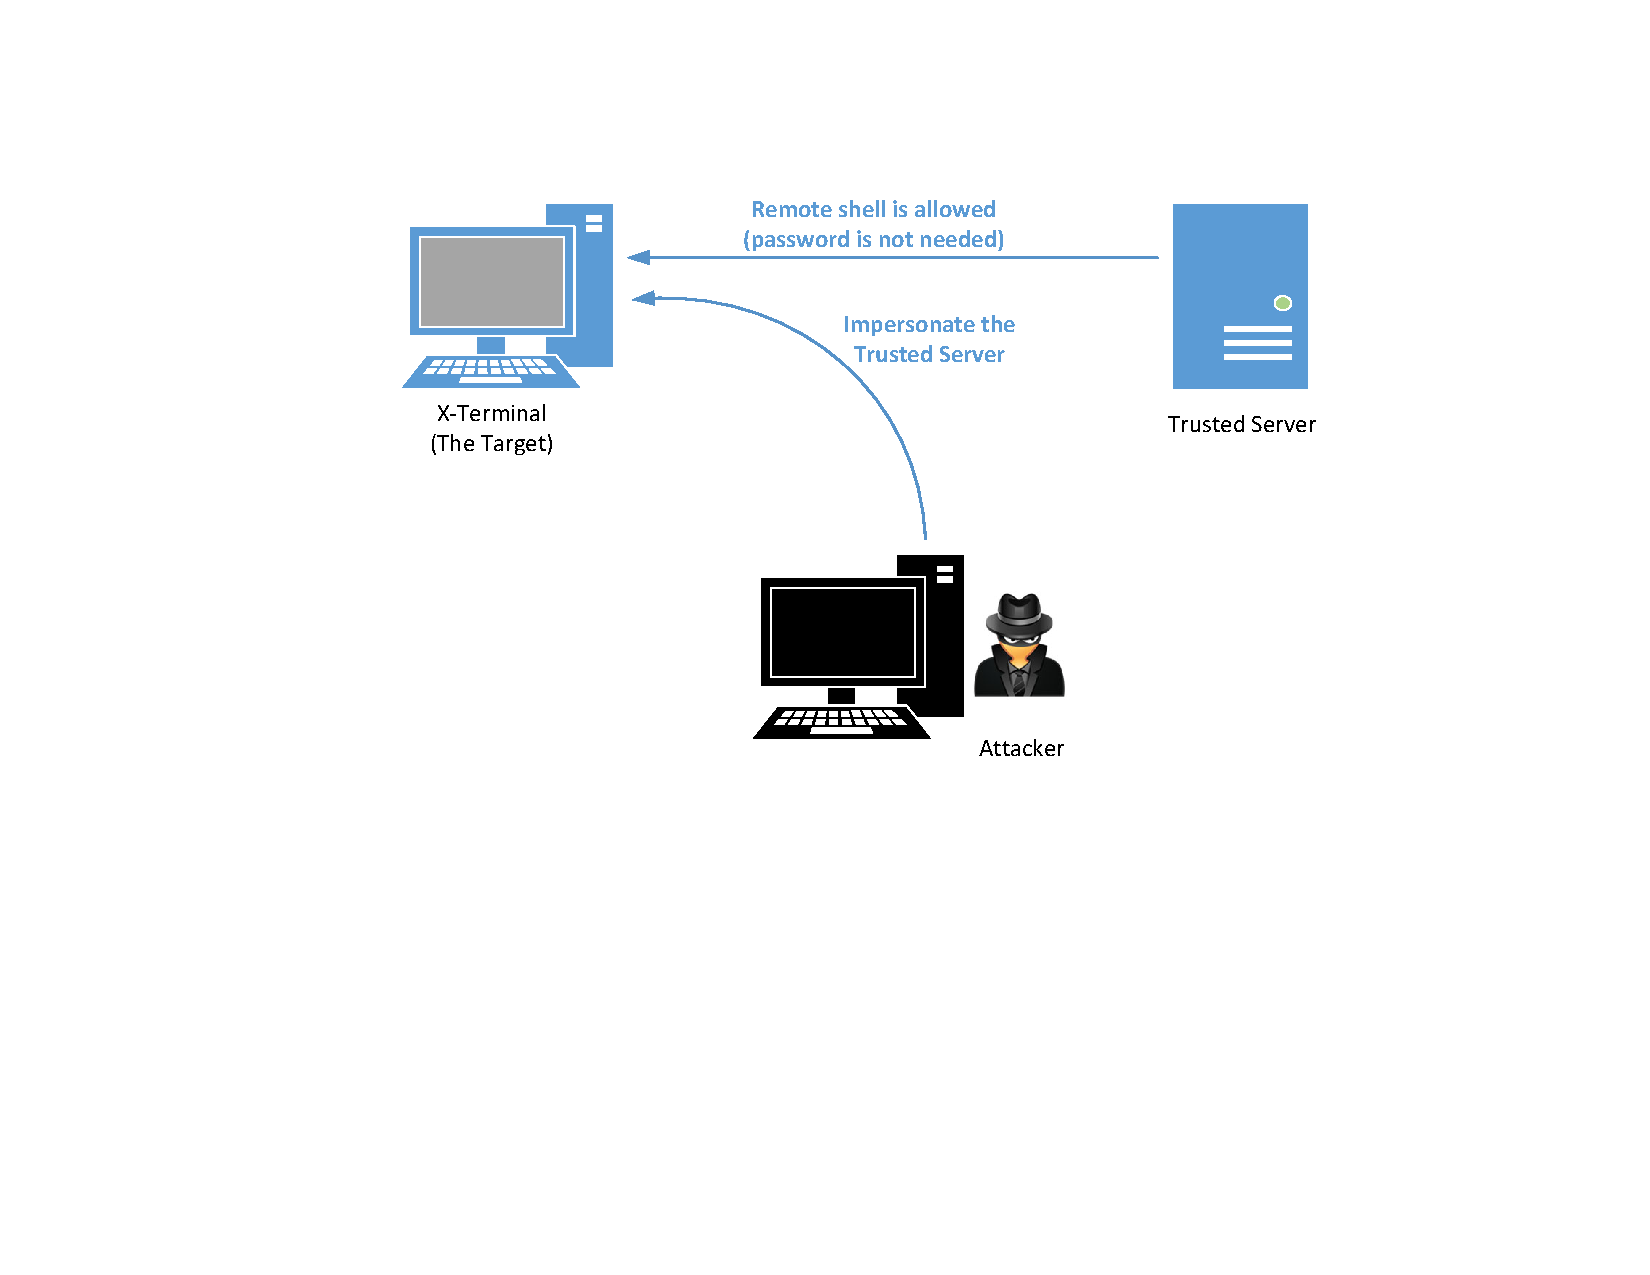
\includegraphics[width=0.8\textwidth]{\mitnickFigs/mitnick_attack.pdf}
\caption{Ilustración del Ataque de Mitnick}
\label{tcp:mitnick}
\end{figure}


\paragraph{Paso 1: Predicción del Número de Secuencia.} 
Antes del ataque, Mitnick necesitaba aprender el patrón del inicio de los números de secuencia (ISN) de la X-Terminal (en esos días los ISN no eran aleatorios).
Mitnick enviaba peticiones SYN a la X-Terminal y recibia respuestas SYN+ACK, entonces enviaba un paquete RESET a la X-Terminal, para así limpiar la cola de half-open connections en esta máquina (esto lo hacía para prevenir que la cola se llene). Después de repetir esto veinte veces. Encontro que había un patrón entre dos TCP ISNs sucesivos. Esto le permitió a Mitnick predecir ISNs, que era un elemento esencial para el ataque.


\paragraph{Paso 2: Ataque de SYN flooding en el Servidor de Confianza.}
Para enviar una petición de conexión desde el Servidor de Confianza hacia la X-Terminal, Mitnick necesitaba enviar un paquete SYN desde el Servidor de Confianza hacia la X-Terminal. Entonces la X-Terminal respondería un paquete SYN+ACK que se enviaría al Servidor de Confianza. Dado que este Servidor de Confianza no era el que iniciaba la petición, enviaría un paquete RESET a la X-Terminal para detener el protcolo de 3-way handshake. Este comportamiento era problemático para el ataque de Mitnick.
Para resolver este problema. Mitnick debía de silenciar al Servidor de Confianza.
Para esto, antes de hacer el spoofing, Mitnick lanzaba un ataque de SYN flooding sobre el servidor. En esa época los servidores eran mucho más vulnerables a este tipo de ataques. El ataque podría dejar a la máquina fuera de servicio, silenciándola por completo.


\paragraph{Paso 3: Spoofear la Conexión TCP.}
Mitnick quería usar \rsh (shell remota o remote shell) para ejecutar un comando a modo de backdoor en la X-Terminal; una vez que el backdoor haya sido instalado, podría loguearse dentro de la X-Terminal.
Para correr una shell remota en la X-Terminal, Mitnick necesitaba poder autenticarse, es de cir necesitaba tener una cuenta válida en la X-Terminal y saber su password. Obviamente, no tenía esta información.

Shimomura solía loguearse a menudo dentro de la X-Terminal desde el Servidor de Confianza. Para evitar tipear el password cada vez que entraba, agregó alguna información en el archivo \texttt{.rhosts}  dentro de la X-Terminal, por lo que al loguearse dentro de la X-Terminal desde el Servidor de Confianza, no se le pediría ningún password. En ese entonces esta era una práctica común. En este escenario Shimomura podía correr cualquier comando en la X-Terminal desde el Servidor de Confianza usando \rsh, or corriendo \texttt{rlogin} para loguearse en la X-Terminal, sin la necesidad de tipear un password.
Mitnick quería explotar esta brecha.

Mitnick necesitaba crear una conexión TCP entre el servidor de confianza y la X-Terminal y luego correr  \rsh dentro de esta conexión
Primero envió una petición SYN hacia la X-Terminal, usando la dirección IP del servidor de confianza como la dirección IP de origen.
La X-Terminal respondió con un SYN+ACK hacia el servidor. Dado que el servidor se encontraba fuera de servicio, no enviaría un RESET para cerrar la conexión. 

Para completar el proceso de 3-way handshake, Mitnick necesitaba spoofear un paquete ACK, que debía de confirmar el número de secuencia en el paquete SYN+ACK de la X-Terminal. Desafortunadamente la respuesta SYN+ACK sólo iba hacia el servidor de confianza y no hacia Mitnick, él no podía ver cual era este número de secuencia. Sin embargo, debido a investigaciones previas, Mitnick podía predecir cual podría ser este número, por lo que podía enviar un paquete ACK spoofeado hacia la X-Terminal para completar el 3-way handshake de forma exitosa.


\paragraph{Paso 4: Correr una shell remota.} 
Usando la conexión TCP establecida entre el servidor de confianza y la X-Terminal, Mitnick podía enviar una petición de shell remota a la X-Terminal, con el objetivo de ejecutar un comando. Usando este comando, Mitnick quería plantar un backdoor en la X-Terminal que le otorgará una shell de forma persistente para no tener que volver a repetir el flujo de ataque.

Todo lo que necesitaba era agregar \texttt{"+ +"} en el archivo \texttt{.rhosts} dentro la X-Terminal.
Pudo hacerlo ejecutando el siguiente comando usando \rsh en la X-Terminal:  {\tt "echo + + > .rhosts"}. 
Dado que los programas \rsh y \texttt{rlogin} usaban el archivo \texttt{.rhosts} para autenticación, con este agregado de Mitnick, X-Terminal confiaría en cualquier petición \rsh y \texttt{rlogin} sin importar de quien sea.


% *******************************************
% SECTION
% ******************************************* 
\section{Setup del Entorno de Laboratorio usando Contenedores}



% -------------------------------------------
% SUBSECTION
% ------------------------------------------- 
\subsection{Setup del Contenedor}

En este laboratorio, necesitamos tres máquinas, una para la X-Terminal, la otra para el Servidor de Confianza y la otra será la del atacante.
En el escenario real del ataque de Mitnick, la máquina del atacante era una máquina remota.
En este laboratorio, por un tema de simplicidad, hemos puesto estas tres máquinas en la misma red.
Los estudiantes pueden usar tres máquina virtuales por separado para hacer el laboratorio, pero es mucho mas conveniente usar los contenedores. 
El entorno de laboratorio se muestra en la Figura \ref{mitnick:fig:labsetup}.


\begin{figure}[htb]
\begin{center}
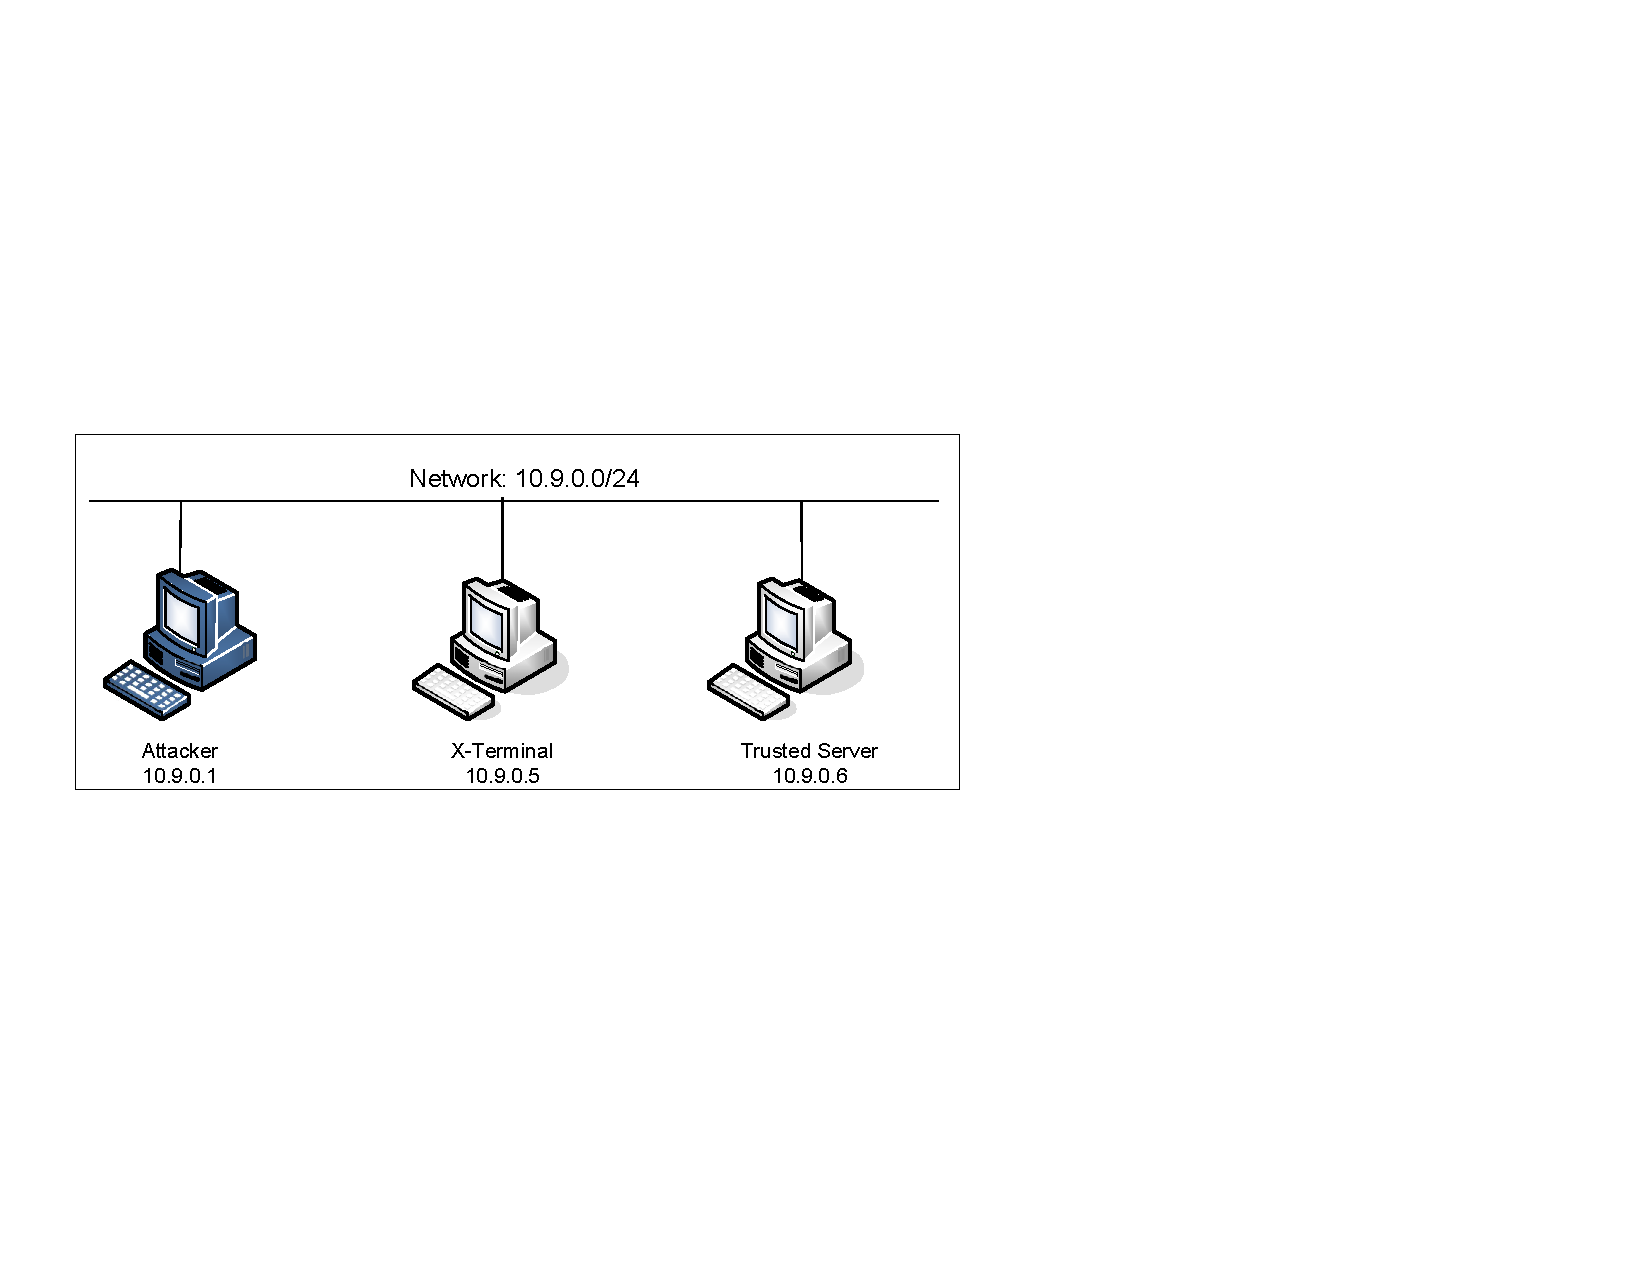
\includegraphics[width=0.8\textwidth]{\commonfolder/Figs/Mitnick_onelan.pdf}
\end{center}
\caption{Setup del Entorno de Laboratorio}
\label{mitnick:fig:labsetup}
\end{figure}
 

%\begin{lstlisting}[backgroundcolor=]
%            +------------+      +--------------+  +----------------+  
%            |     VM     |      |   Container  |  |    Container   |  
%            | (attacker) |      | (X-Terminal) |  |(Trusted Server)|  
%            |  10.9.0.1  |      |   10.9.0.5   |  |    10.9.0.6    |  
%            +----+-------+      +-------+------+  +--------+-------+  
%                 | br-<id>             | eth0          | eth0   
%                 |                     |               |        
%           ------+---------------------+---------------+--------------
%           Network  10.9.0.0/24
%
%\end{lstlisting}



% -------------------------------------------
% SUBSECTION
% -------------------------------------------
\subsection{Setup del Contenedor y sus Comandos}

%%%%%%%%%%%%%%%%%%%%%%%%%%%%%%%%%%%%%%%%%%%%
Para empezar a preparar el contenedor, deberá descargarse el archivo \texttt{Labsetup.zip} ubicado en el laboratorio correspondiente dentro del sitio web oficial y copiarlo dentro de la Máquina Virtual prevista por SEED. Una vez descargado deberá descomprimirlo y entrar dentro del directorio \texttt{Labsetup} donde encontrará el archivo \texttt{docker-compose.yml} que servirá para setear el entorno de laboratorio. Para una información más detallada sobre el archivo \texttt{Dockerfile} y otros archivos relacionados, puede encontrarla dentro del Manual de Usuario del laboratorio en uso, en el sitio web oficial de SEED.

Si esta es su primera experiencia haciendo el setup del laboratorio usando contenedores es recomendable que lea el manual anteriormente mencionado.

A continuación, se muestran los comandos más usados en Docker y Compose.
Debido a que estos comandos serán usados con mucha frecuencia, hemos creados un conjunto de alias para los mismos, ubicados en del archivo \texttt{.bashrc} dentro de la Máquina Virtual provista por SEED (Ubuntu 20.04)

\begin{lstlisting}
$ docker-compose build  # Build the container image
$ docker-compose up     # Start the container
$ docker-compose down   # Shut down the container

// Aliases for the Compose commands above
$ dcbuild       # Alias for: docker-compose build
$ dcup          # Alias for: docker-compose up
$ dcdown        # Alias for: docker-compose down
\end{lstlisting}


Dado que todos los contenedores estarán corriendo en un segundo plano. Necesitamos correr comandos para interactuar con los mismos, una de las operaciones fundamentales es obtener una shell en el contenedor. 
Para este propósito usaremos \texttt{"docker ps"} para encontrar el ID del contenedor deseado y ingresaremos \texttt{"docker exec"} para correr una shell en ese contenedor.
Hemos creado un alias para ello dentro del archivo \texttt{.bashrc}

\begin{lstlisting}
$ dockps        // Alias for: docker ps --format "{{.ID}}  {{.Names}}" 
$ docksh <id>   // Alias for: docker exec -it <id> /bin/bash

// The following example shows how to get a shell inside hostC
$ dockps
b1004832e275  hostA-10.9.0.5
0af4ea7a3e2e  hostB-10.9.0.6
9652715c8e0a  hostC-10.9.0.7

$ docksh 96
root@9652715c8e0a:/#  

// Note: If a docker command requires a container ID, you do not need to 
//       type the entire ID string. Typing the first few characters will 
//       be sufficient, as long as they are unique among all the containers. 
\end{lstlisting}

En caso de problemas configurando el entorno, por favor consulte la sección ``Common Problems'' en el manual ofrecido por SEED. 


%%%%%%%%%%%%%%%%%%%%%%%%%%%%%%%%%%%%%%%%%%%%



% -------------------------------------------
% SUBSECTION
% -------------------------------------------
\subsection{Sobre el Contenedor del Atacante}

I
Para este laboratorio podemos usar tanto una Máquina Virtual como un contenedor como máquina de ataque. Si observa el archivo Docker Compose, verá que el contenedor de ataque está configurado de forma
diferente al resto de los contenedores.

\begin{itemize}
\item \textit{Directorio Compartido.} Cuando usemos el contenedor del atacante para realizar los ataques, necesitamos poner el código de ataque dentro del contenedor.
%%%%%%%%%%%%%%%%%%%%%%%%%%%%%%%%%%%%%%%%%%%%%%%
Code editing is more convenient inside the VM than in containers, 
because we can use our favorite editors.
In order for the VM and container to share files, 
we have created a shared folder between the VM and the container
using the Docker \texttt{volumes}.
If you look at the Docker Compose file, you will find out that
we have added the following entry to some of the containers.
It indicates mounting the \texttt{./volumes} folder on the host
machine (i.e., the VM) to the \texttt{/volumes} folder inside the container.
We will write our code in the \texttt{./volumes} folder (on the VM), so they
can be used inside the containers.

\begin{lstlisting}
volumes:
       - ./volumes:/volumes
\end{lstlisting}


%%%%%%%%%%%%%%%%%%%%%%%%%%%%%%%%%%%%%%%%%%%%%%%

\item \textit{Host Mode.}
%%%%%%%%%%%%%%%%%%%%%%%%%%%%%%%%%%%%%%%%%%%%%%%
In this lab, the attacker needs to be able to sniff packets,
but running sniffer programs inside a container has problems, because
a container is effectively attached to a virtual switch, 
so it can only see its own traffic, and it is never going to see 
the packets among other containers. To solve this problem,
we use the \texttt{host} mode for the attacker container. This
allows the attacker container to see all the traffics. The following
entry used on the attacker container:

\begin{lstlisting}
network_mode: host
\end{lstlisting}

When a container is in the \texttt{host} mode,  it sees
all the host's network interfaces, and it even has the same
IP addresses as the host. Basically, it is put in the
same network namespace as the host VM. However, the container
is still a separate machine, because its other namespaces are
still different from the host.


%%%%%%%%%%%%%%%%%%%%%%%%%%%%%%%%%%%%%%%%%%%%%%%


\item \textit{Privileged Mode.}
%%%%%%%%%%%%%%%%%%%%%%%%%%%%%%%%%%%%%%%%%%%%%%%
Para poder modificar parámetros del kernel en tiempo de ejecución (usando  \texttt{sysctl}), tal como IP forwarding, el contenedor debe de ser privilegiado.
Esto se consigue incluyendo la siguiente entrada dentro del archivo Docker compose del contenedor.

\begin{lstlisting}
privileged: true
\end{lstlisting}


%%%%%%%%%%%%%%%%%%%%%%%%%%%%%%%%%%%%%%%%%%%%%%%

\end{itemize}


% -------------------------------------------
% SUBSECTION
% ------------------------------------------- 
\subsection{Instalando \rsh}

Remote shell \rsh es un programa de consola que sirve para ejecutar comandos shell de manera remota. Aunque usaremos \rsh en esta tarea, deberíamos de saber que \rsh y \texttt{rlogin} no son seguros y ya no se usan mas.
Han sido reemplazados por programas más seguros como \texttt{ssh}.
Debido a esto en los sistemas operativos linux actuales, el comando \rsh es un link simbólico al programa \texttt{ssh}.

\begin{lstlisting}
$ ls -al /etc/alternatives | grep rsh
lrwxrwxrwx   1 root root    12 Jul 25  2017 rsh -> /usr/bin/ssh
\end{lstlisting}

Para recrear el ataque de Mitnick, necesitamos instalar la version insegura del programa \rsh. Obviamente la vieja versión de\ \rsh ya no funciona, pero existe un proyecto de código abierto que implementa el cliente y el servidor remoto de shell.
Podemos usar los siguientes comandos para instalar el servidor y el cliente \rsh:
\textbf{Nota:} Los programas \rsh ya fueron instalados en los contenedores X-Terminal y el Servidor de Confianza (vea dentro del archivo \texttt{Dockerfile} dentro del directorio de las imágenes).

\begin{lstlisting}
$ sudo apt-get install rsh-redone-client
$ sudo apt-get install rsh-redone-server
\end{lstlisting}




% -------------------------------------------
% SUBSECTION
% ------------------------------------------- 
\subsection{Configuración}
\label{subsec:configuration}

El servidor \rsh usa dos archivos para autenticación, \texttt{.rhosts} y \texttt{/etc/hosts.equiv}.
Cada vez que el servidor recibe una petición de comando de manera remota, chequeará the \texttt{/etc/hosts.equiv}. Si la petición proviene de un hostname que se encuentra dentro de este archivo, el servidor la aceptará sin pedir password.
Si  \texttt{/etc/hosts.equiv} no existe o no contiene ese hostname, \rsh chequeará el archivo \texttt{.rhosts} en el directorio home del usuario.

Shimomura necesitaba correr con frecuencia comandos remotos en la X-Terminal desde el servidor de confianza. Para evitar ingresar un password cada vez que le era necesario, creo el archivo \texttt{.rhosts} en la X-Terminal y puso la dirección IP del servidor dentro del mismo.
Note que el archivo \texttt{.rhosts} debe de ubicarse en la raíz del directorio home del usuario y puede ser escrito solamente por el \textbf{usuario propietario}.

Por favor ejecute los siguientes comandos en la X-Terminal para hacer el setup del archivo \texttt{.rhosts}.
Cabe señalar que cuando entramos en este contenedor, lo haremos con una cuenta de root. En este laboratorio necesitamos cambiar a una cuenta de usuario normal llamada seed, que fue creada dentro del contenedor:

\begin{lstlisting}
# su seed          (*@\reflectbox{\ding{217}}@*) Switch to the seed account
$ cd               (*@\reflectbox{\ding{217}}@*) Go to seed's home directory
$ touch .rhosts    (*@\reflectbox{\ding{217}}@*) Create an empty file 
$ echo [Server's IP address] > .rhosts
$ chmod 644 .rhosts
\end{lstlisting}

Para verificar su configuración, intente ejecutar el siguiente comando en el servidor de confianza.
\begin{lstlisting}
# su seed          (*@\reflectbox{\ding{217}}@*) Switch to the seed account
$ rsh [X-Terminal's IP] date
\end{lstlisting}

Si el comando despliega en pantalla la fecha y hora actual, su configuración esta funcionando. Si ud. ve  ``Authentication Failure'', quiere decir que fue mal configurado.
Un error común es el permiso en el archivo \texttt{.rhosts}: debería de asegurarse que solamente el usuario propietario posea permisos de escritura sobre el mismo.

\paragraph{Permitir a Todos.} Para hacer que cualquier usuario con cualquier dirección IP pueda ejecutar comandos en la X-Terminal, necesitamos poner dos signos de suma (\texttt{"+ +"}) dentro del archivo \texttt{.rhosts}. Esto es algo peligroso y nadie debería de hacerlo. Pero si ud. es el atacante, es una forma conveniente de setear un backdoor. Como hemos mencionado anteriormente, esto es lo que se usó en el ataque de Mitnick.


% *******************************************
% SECTION
% ******************************************* 
\section{Tarea 1: SYN flooding Simulado}

En la época del ataque de Mitnick, los sistemas operativos eran vulnerables a ataques de SYN flooding, que ocasionaban que una máquina remota quede fuera de servicio o sin responder.
Hoy en día con el avance de los sistemas operativos modernos, los ataques de SYN flooding no causan semejante daño.
Haremos una simulación de los daños de este tipo de ataque.

Podemos detener el contenedor del servidor de confianza manualmente, pero eso no es suficiente.
Cuando la X-Terminal recibe un paquete SYN del servidor de confianza, responderá con un paquete SYN+ACK. Antes de enviar este paquete, necesita saber la dirección MAC del servidor de confianza.
La caché ARP será chequeada primero. Si no existe ninguna entrada para el servidor de confianza, la X-Terminal enviará un petición ARP para preguntar por esa dirección MAC. Dado que el servidor confianza ha sido silenciado, nadie va a responder esa petición ARP, por ende X-Terminal no podrá enviar la respuesta. Como resultado la conexión TCP no podrá ser establecida.

En el ataque real, la dirección MAC del servidor de confianza se encontraba dentro de la caché ARP de la X-Terminal. Incluso si no lo estaba, antes de dejar inhabilitado al servidor de confianza, podíamos spoofear una petición echo ICMP desde el servidor de confianza hacia la X-Terminal, lo que haría que la X-Terminal respondiera al servidor de confianza y obtendríamos la dirección MAC del mismo y la guardaríamos en la caché.

Para simplificar la tarea, antes de detener el servidor de confianza, haremos un ping de la X-Terminal una sola vez, y usaremos el comando \texttt{arp} para asegurarnos que la dirección MAC se encuentre en la caché. Cabe señalar que esta entrada puede ser removida por el sistema operativo si este falla a la hora encontrar el destino usando la dirección MAC que está en la caché. Para simplificar su ataque, puede ejecutar el siguiente comando en la X-Terminal para agregar una entrada de manera permanente en la caché ARP (necesita hacerlo como usuario root):

\begin{lstlisting}
# arp -s [Server's IP] [Server's MAC]
\end{lstlisting}



% *******************************************
% SECTION
% ******************************************* 
\section{Tarea 2: Spoofear Conexiones TCP y Sesiones \rsh}
\label{sec:task2}

Ahora que hemos ``desactivado'' al servidor de confianza, podemos suplantarlo y tratar de lanzar una sesión \rsh con X-Terminal. Dado que \rsh corre sobre TCP, primero necesitamos establecer una conexión TCP entre el servidor de confianza y la X-Terminal y recién después correr \rsh sobre esta conexión.

Una de las dificultades en el ataque de Mitnick es predecir los números de secuencia TCP.
En aquel tiempo era posible cuando los números de secuencia TCP no eran generados de forma aleatoria.
Hoy en día los sistemas operativos randomizan los números de secuencia TCP (como medida de protección contra ataques de TCP session hijacking), por lo que predecirlos se vuelve imposible.
Para simular la situación del ataque original, los estudiantes pueden sniffear los paquetes y obtener los números de secuencia, en vez de adivinarlos.


\paragraph{Restricción.} Para poder simular el ataque original de Mitnick lo más parecido posible al que fue en ese tiempo, aunque los estudiantes pueden sniffear paquetes TCP de la X-Terminal, no pueden usar todos los campos de estos paquetes, porque en los ataques reales Mitnick no pudo sniffear paquetes. Cuando los estudiantes escriban sus programas de ataque, solamente podrán usar los siguientes campos de los paquetes capturados, de forma contraria se aplicará una pena.


\begin{itemize}
\item \textbf{Campo de Número de Secuencia TCP} (Esto no incluye el campo de Acknowledgment).

\item \textbf{Campo flag TCP}. Este nos permite saber que tipo de paquete TCP es. En el ataque real de Mitnick, Mitnick sabía que tipo de paquetes eran enviados por la X-Terminal, porque eran parte del protocolo de 3way-handshake. Para simplificar el ataque se les permite a los estudiantes usar este campo.


\item \textbf{Todos los campos de Longitud}, incluídos el campo de longitud del encabezado IP, la longitud total IP y la longitud del encabezado TCP. Estas piezas de información no son necesarias para los ataques. En el ataque de Mitnick , Mitnick sabía exactamente cuales eran estos valores. Para simplificar el ataque se les permite a los estudiantes usar estos campos.
\end{itemize}


\paragraph{El Comportamiento \rsh.} 
Para crear una sesión \rsh spoofeada entre el servidor de confianza y la X-Terminal, necesitamos entender el comportamiento de \rsh. Vamos a crear una sesión \rsh desde el servidor de confianza hacia la X-Terminal y usaremos Wireshark para capturar los paquetes enviados entre ellos (nota: correremos Wireshak desde la máquina virtual del atacante; asegurése de seleccionar la interfaz de red correcta que corresponde a la red \texttt{10.9.0.0/24}).
Usamores el siguiente comando para ejecutar el comando \texttt{date} en el Host B desde el Host A a través de \rsh.

\begin{lstlisting}
// On Trusted Server
$ rsh 10.9.0.5 date
\end{lstlisting}

El packet trace de la sesión \rsh es motrado a continuación.
En este entorno  \texttt{10.9.0.6} es la dirección IP del servidor de confianza y \texttt{10.9.0.5} es la dirección IP de la X-Terminal.
Si el paquete no lleva ningún dato TCP, la información de longitud (es decir \texttt{Len=0}) es omitida.

\begin{lstlisting}[caption={Packet trace de una sesión \rsh},
                  label={listing:rsh}]
# The first connection
   SRC IP    DEST IP   TCP Header
1  10.9.0.6  10.9.0.5  1023 -> 514 [SYN] Seq=778933536 
2  10.9.0.5  10.9.0.6  514 -> 1023 [SYN,ACK] Seq=10879102 Ack=778933537 
3  10.9.0.6  10.9.0.5  1023 -> 514 [ACK] Seq=778933537 Ack=10879103 
4  10.9.0.6  10.9.0.5  1023 -> 514 [ACK] Seq=778933537 Ack=10879103 Len=20
                       RSH Session Establishment
                       Data: 1022\x00seed\x00seed\x00date\x00
5  10.9.0.5  10.9.0.6  514 -> 1023 [ACK] Seq=10879103 Ack=778933557

# The second connection
6  10.9.0.5  10.9.0.6  1023 -> 1022 [SYN] Seq=3920611526 
7  10.9.0.6  10.9.0.5  1022 -> 1023 [SYN,ACK] Seq=3958269143 Ack=3920611527 
8  10.9.0.5  10.9.0.6  1023 -> 1022 [ACK] Seq=3920611527 Ack=3958269144 


# Going back to the first connection
9  10.9.0.5  10.9.0.6  514 -> 1023 [ACK] Seq=10879103 Ack=778933557 Len=1
                       Data: \x00
10 10.9.0.6  10.9.0.5  1023 -> 514 [ACK] Seq=778933557 Ack=10879104 
11 10.9.0.5  10.9.0.6  514 -> 1023 [ACK] Seq=10879104 Ack=778933557 Len=29
                       Data: Sun Feb 16 13:41:17 EST 2020
\end{lstlisting}

Podemos observar que una sesión \rsh consiste en dos conexiones TCP.
La primera conexión es iniciada por el Host A (el cliente).
El proceso \texttt{rshd} en el Host B está a la escucha de peticiones entrantes en el puerto 514.
Los paquetes del 1 a 3 son para del protocolo del 3way-handshake.
Después de que la conexión ha sido establecida, el cliente envía los datos \rsh (incluídos los IDs de usuario y los comandos) al Host B (paquete 4).
El proceso \texttt{rshd} autenticará al usuario y si este es autenticado de forma exitosa, \texttt{rshd} inicia una conexión TCP separada con el cliente.

La segunda conexión es usada para enviar mensajes de error.
En la traza anterior, dado que no hubo errores, esta conexión nunca fue usada, pero la conexión debe ser establecida o  \texttt{rshd} no podrá continuar. Los paquetes del 6 al 7 son para el protocolo de 3way-handshake de la segunda conexión.

Después de que la segunda conexión ha sido establecida, el Host B enviará un zero byte al cliente (usando la primera conexión) el Host A aceptará este paquete. Después de eso, el proceso  \texttt{rshd} en el Host B ejecutará el comando enviado por el cliente y su salida será enviada de regreso al cliente, usando la primera conexión.
Los estudiantes pueden usar Wireshak para capturar la sesión \rsh y estudiar sus comportamientos antes de lanzar el ataque de Mitnick.
Hemos dividido el ataque en dos sub-tareas, cada una se centra en una conexión.



% -------------------------------------------
% SUBSECTION
% ------------------------------------------- 
\subsection{Tarea 2.1: Spoofear la primera Conexión TCP}
\label{sec:first-conn}

The first TCP connection is initiated by the attacker via a spoofed SYN packet. As you can see
in Figure~\ref{fig:first-conn}, after X-Terminal receives the SYN packet, it will in turn send
a SYN+ACK packet to the trusted server. Since the server has been brought down, it will not
reset the connection. The attacker, which is on the same network, can sniff the packet and get
the sequence number.

\begin{figure}[htb]
\centering
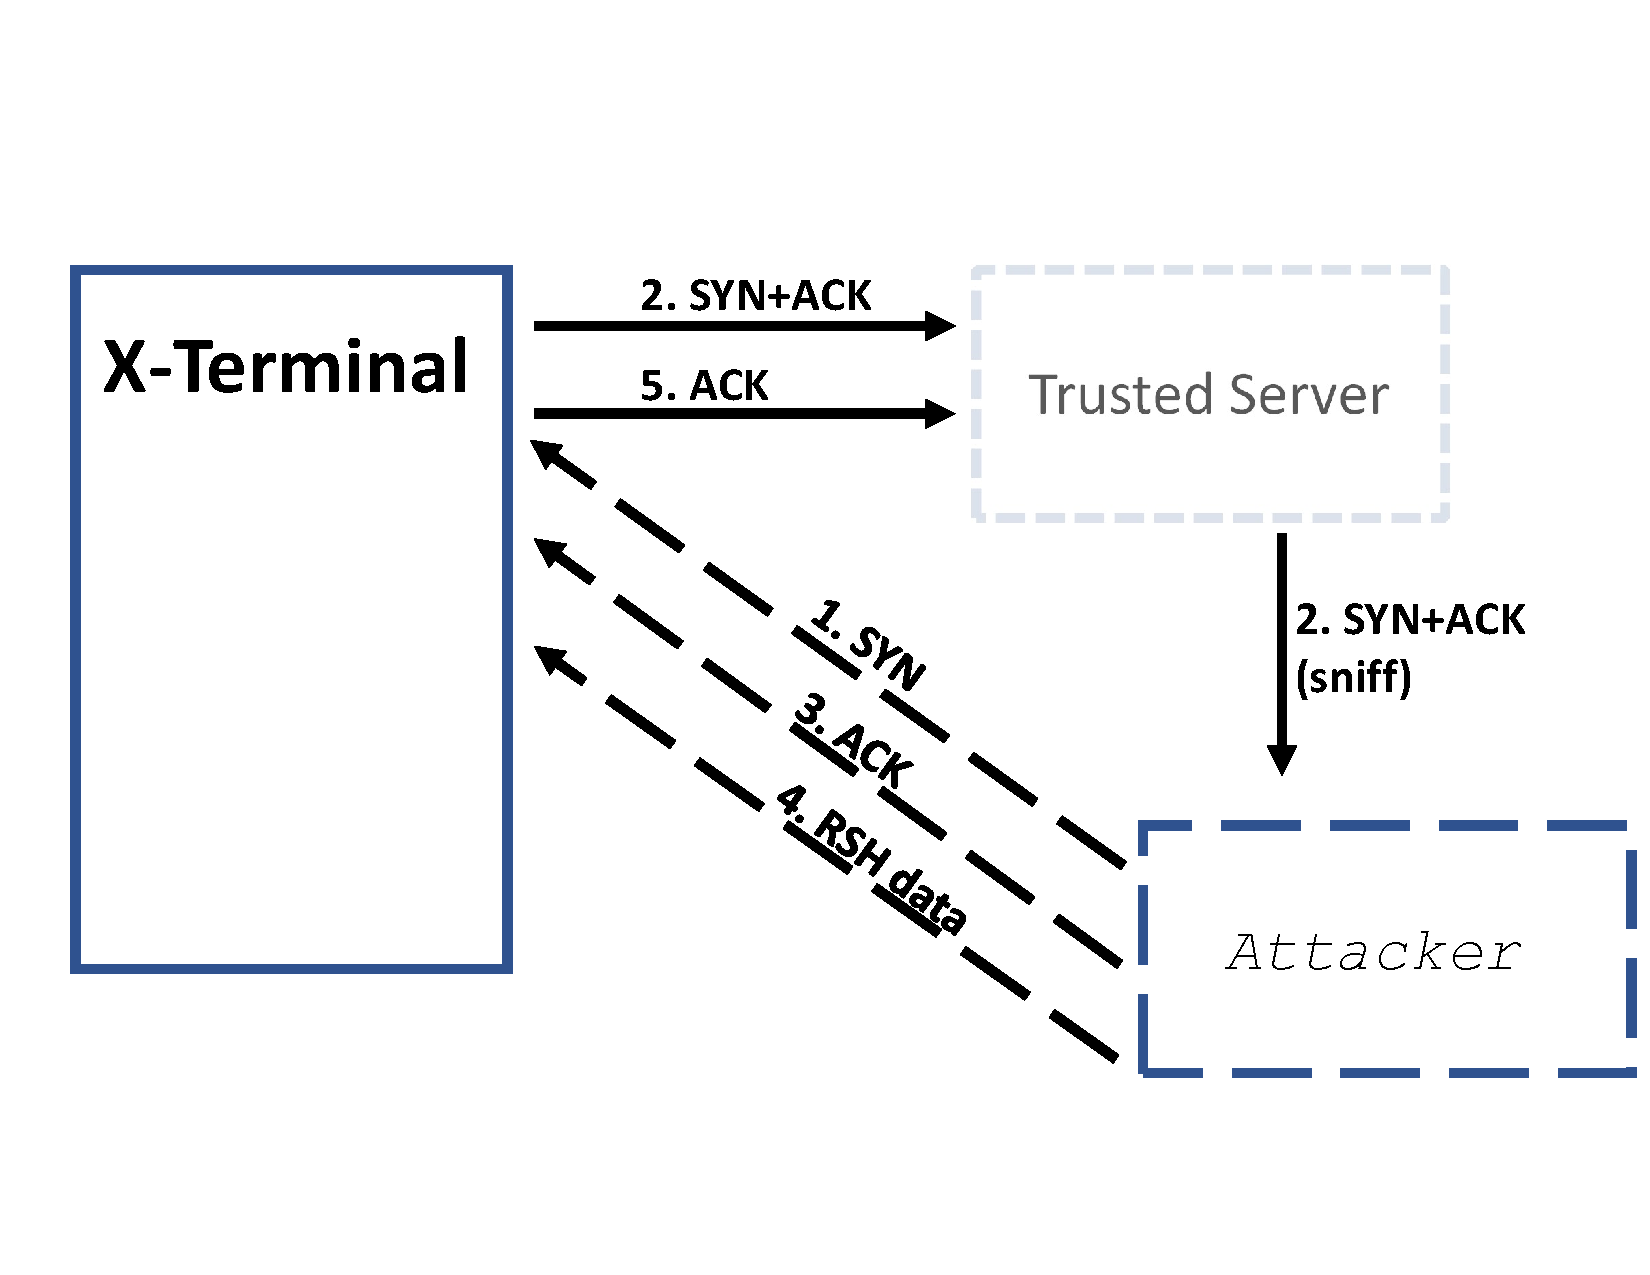
\includegraphics[width=0.6\textwidth]{\mitnickFigs/mitnick-diagram-1.pdf}
\caption{First Connection}
\label{fig:first-conn}
\end{figure}


\paragraph{Paso 1: Spoofear un paquete SYN.}
Students should write a program to spoof a SYN packet 
from the trusted server to X-Terminal (see Packet 1 in Listing~\ref{listing:rsh}). 
There are six standard 
TCP code bits, and they can be set in the flag field of the TCP header. 
The following code examples show how to set the flag field
and how to check whether certain bits are set in
the flag field. 

\begin{lstlisting}
# 'U': URG bit
# 'A': ACK bit
# 'P': PSH bit
# 'R': RST bit
# 'S': SYN bit
# 'F': FIN bit

tcp = TCP()

# Set the SYN and ACK bits
tcp.flags = "SA"

# Check whether the SYN and ACK are the only bits set
if tcp.flags == "SA": 

# Check whether the SYN and ACK bits are set
if 'S' in tcp.flags and 'A' in tcp.flags: 
\end{lstlisting}

It should be noted that the source port of the SYN packet 
must be from port \texttt{1023}. If a different port 
is used, \rsh will reset the connection 
after the connection is established.  If this step is successful, 
from Wireshark, we should be
able to see a SYN+ACK packet coming out of 
X-Terminal (see Packet 2 in Listing~\ref{listing:rsh}).


\paragraph{Paso 2: Responder al paquete SYN+ACK.}
After X-Terminal sends out a SYN+ACK, the trusted server needs 
to send out an ACK packet to complete the three-way handshake protocol. 
The acknowledge number in the packet should be \texttt{S+1}, where 
\texttt{S} is the sequence number contained in the SYN+ACK packet. 
See Packet 3 in Listing~\ref{listing:rsh}.

In the actual Mitnick attack, the attacker could not see the SYN+ACK packet, because
it was sent to the trusted server, not to the attacker. 
That is why Mitnick had to guess the value of the sequence number.
In this lab, we allow students to get 
the sequence number via packet sniffing. 

Students need to write a sniff-and-spoof program using \texttt{Scapy} and run it
on the attacker's machine. Here is a skeleton of a sniff-and-spoof program that might be
useful. Please make sure to follow the restrictions described at the
beginning of the section, or you will get a penalty. 


\begin{lstlisting}
#!/usr/bin/python3
from scapy.all import *

x_ip      = "10.9.0.5"  # X-Terminal
x_port    = 514         # Port number used by X-Terminal

srv_ip    = "10.9.0.6"  # The trusted server
srv_port  = 1023        # Port number used by the trusted server

# Add 1 to the sequence number used in the spoofed SYN
seq_num     = 0x1000 + 1


def spoof(pkt):
  global seq_num   # We will update this global variable in the function

  old_ip  = pkt[IP]
  old_tcp = pkt[TCP]

  # Print out debugging information
  tcp_len = old_ip.len - old_ip.ihl*4 - old_tcp.dataofs*4  # TCP data length
  print("{}:{} -> {}:{}  Flags={} Len={}".format(old_ip.src, old_tcp.sport,
                         old_ip.dst, old_tcp.dport, old_tcp.flags, tcp_len))



  # Construct the IP header of the response
  ip = IP(src=srv_ip, dst=x_ip)

  # Check whether it is a SYN+ACK packet or not;
  #   if it is, spoof an ACK packet

  # ... Add code here ...

myFilter = 'tcp'   # You need to make the filter more specific
sniff(iface='br-****', filter=myFilter, prn=spoof)
                  (*@\reflectbox{\ding{218}} \textbf{You need to set the correct value here.}@*)   
\end{lstlisting}




\paragraph{Paso 3: Spoofear el paquete de datos de \rsh.}
Once the connection is established, the attacker needs to 
send \rsh data to X-Terminal.
The structure of the \rsh data is shown below.

\begin{lstlisting}
[port number]\x00[uid_client]\x00[uid_server]\x00[your command]\x00
\end{lstlisting}

The data has four parts: a port number, client's user ID, server's user ID,
and a command.
The port number will be used for the second connection (see Task 2.2). 
Both client and server's user ID is \texttt{seed} in our container. 
The four fields are separated by a byte 0.
Note that there is also a byte 0 at the end of the \rsh data. An example is given in the
following. In this example, we tell X-Terminal that we are going to listen on port 9090 for the
second connection and the command we want to run is \texttt{"touch /tmp/xyz"}. 

\begin{lstlisting}
data = '9090\x00seed\x00seed\x00touch /tmp/xyz\x00'
send(IP()/TCP()/data, verbose=0)
\end{lstlisting}
 

Students should modify the sniff-and-spoof program written in Step 2, so
an \rsh data packet is sent to X-Terminal (see Packet 4 
in Listing~\ref{listing:rsh}). 
If this step is successful, from Wireshark, we can see
that X-Terminal is going to initiate a TCP connection to the trusted server's port
\texttt{9090}, which is the port number specified in our \rsh data.  

In your report, please describe whether the \texttt{touch} command 
has been executed on X-Terminal or not. Please also 
include snapshots of your Wireshark. 


% -------------------------------------------
% SUBSECTION
% ------------------------------------------- 
\subsection{Paso 2.2: Spoofear la segunda Conexión TCP}
\label{sec:second-conn}

\begin{figure}[htb]
\centering
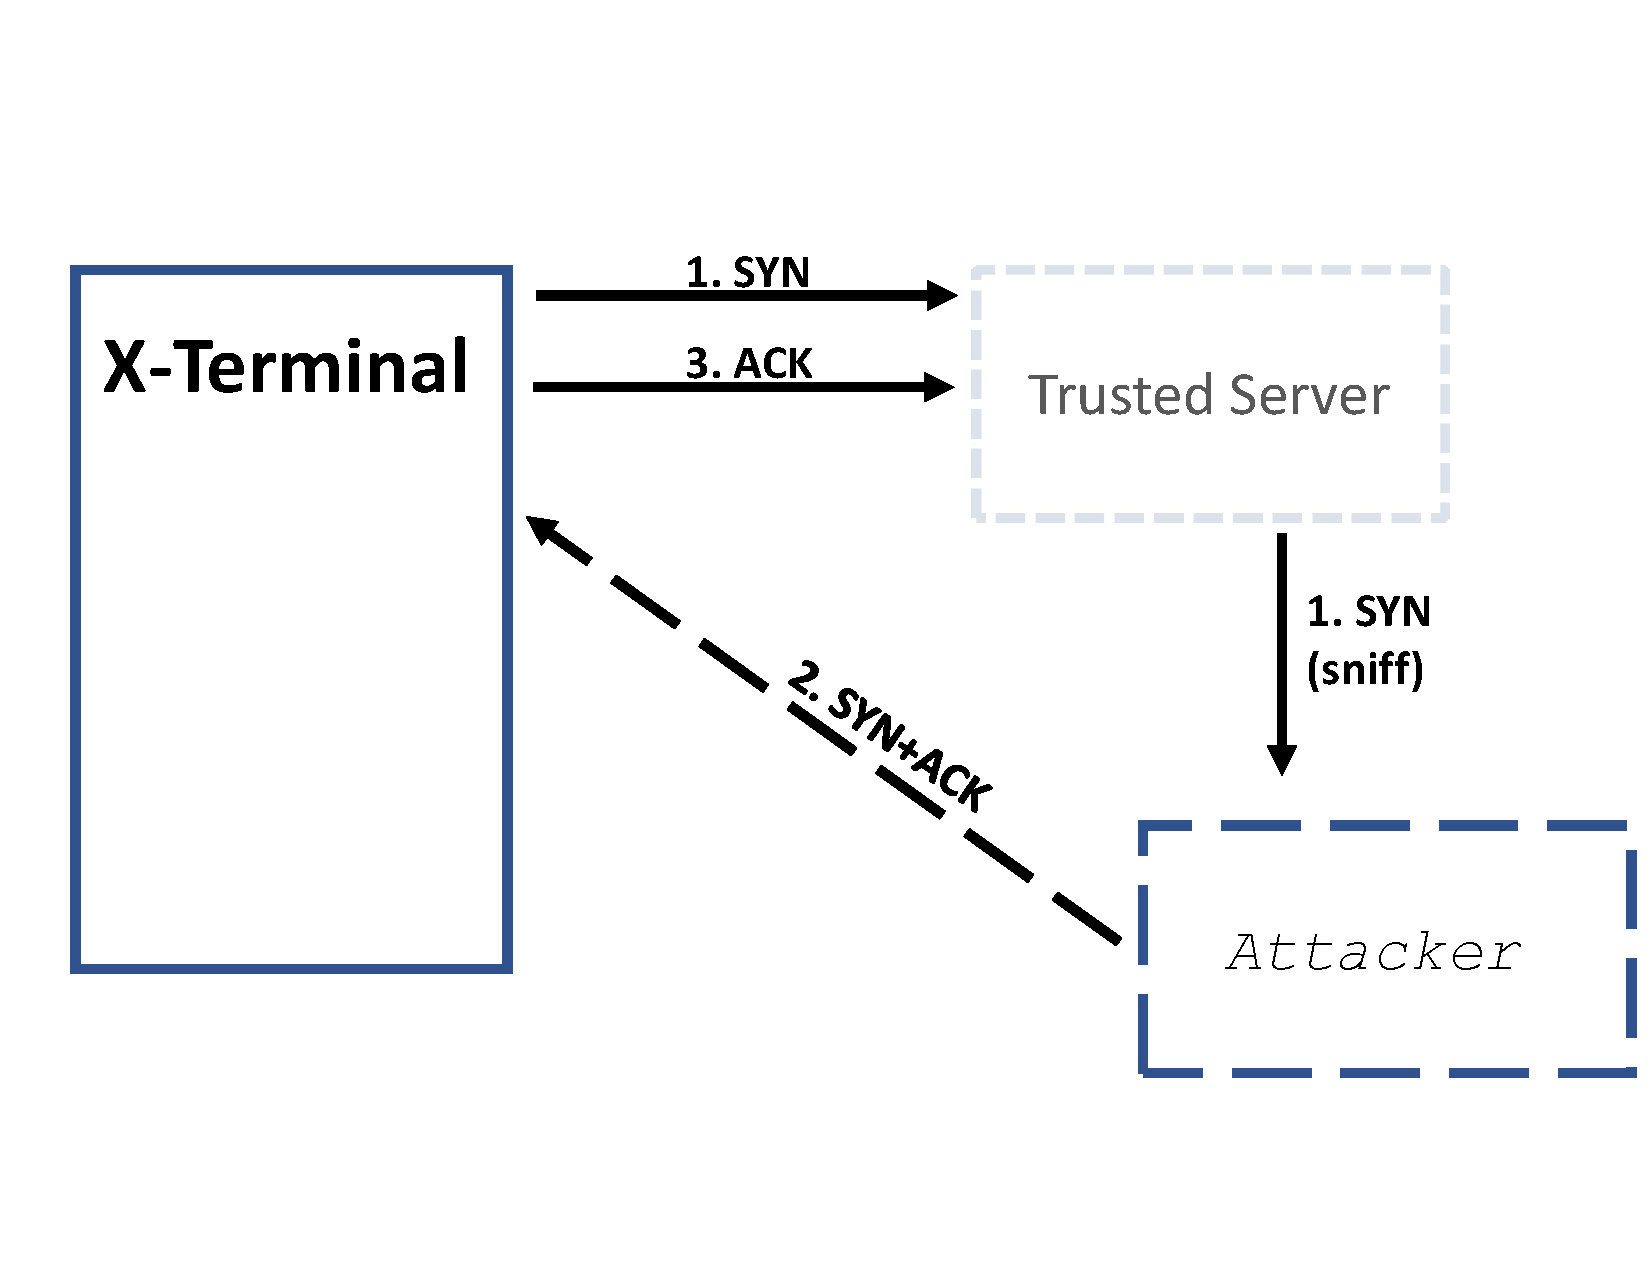
\includegraphics[width=0.6\textwidth]{\mitnickFigs/mitnick-diagram-2.pdf}
\caption{Second Connection}
\label{fig:second-conn}
\end{figure}


After the first connection has been established, X-Terminal will initiate 
the second connection. This connection is used by \texttt{rshd} to send 
out error messages. In our attack, we will not use this connection, but
if this connection is not established, \texttt{rshd} will stop without 
executing our command. Therefore, we need to use spoofing 
to help X-Terminal and the trusted server finish establishing this connection. 
See Figure~\ref{fig:second-conn}. 


Students need to write another sniff-and-spoof program, which
sniffs the TCP traffic going to the port 9090 of the trusted server (assuming
\texttt{9090} is used in Task 2.1). When it sees a SYN packet,
it should respond with a SYN+ACK packet. See Packet 7 
in Listing~\ref{listing:rsh} for an example.

If both connections have been successfully established, \texttt{rshd} 
will execute the command contained in the \rsh data packet. Please 
check the \texttt{/tmp} folder and see whether \texttt{/tmp/xyz} is created
and whether its timestamp matches the present time. Please 
include your evidence in your report. 



% *******************************************
% SECTION
% ******************************************* 
\section{Tarea 3: Plantar el Backdoor}

In Task 2, we only run a \texttt{touch} command in the attack to prove that we can
successfully run a command on X-Terminal. If we want to run
more commands later, we can always launch the same attack. That is quite inconvenient. 

Mitnick did plan to come back to X-Terminal. Instead of launching the attack
again and again, he planted a backdoor in X-Terminal after his initial attack. 
This backdoor allowed him to log into X-Terminal normally anytime he wanted, without 
typing any password. 
To achieve this goal, as we have discussed in 
Section~\ref{subsec:configuration}, 
all we need to do is to add the string \texttt{"+ +"} to
the \texttt{.rhosts} file (in a single line). We can
include the following command in our \rsh data.

\begin{lstlisting}
echo + + > .rhosts
\end{lstlisting}

Students should replace the \texttt{touch} command in Task 2 with
the \texttt{echo} command above, and then repeat the attack.   
If the attack succeeds, the attacker should be able to 
remotely log into X-Terminal using the following command,
and no password is needed: 

\begin{lstlisting}
$ rsh [X-Terminal's IP]
\end{lstlisting}

The \texttt{rsh} program may have not been installed on the attacker container, 
but you can easily install it using the following commands:

\begin{lstlisting}
# apt-get update && apt-get -y install rsh-redone-client 
\end{lstlisting}


% *******************************************
% SECTION
% ******************************************* 
\section{Informe del Laboratorio}


%%%%%%%%%%%%%%%%%%%%%%%%%%%%%%%%%%%%%%%%

Debe enviar un informe de laboratorio detallado, con capturas de pantalla, para describir lo que ha hecho y lo que ha observado.
También debe proporcionar una explicación a las observaciones que sean interesantes o sorprendentes.
Enumere también los fragmentos de código más importantes seguidos de una explicación. No recibirán créditos aquellos fragmentos de códigos que no sean explicados.
%%%%%%%%%%%%%%%%%%%%%%%%%%%%%%%%%%%%%%%%

\section*{Agradecimientos}

Este documento ha sido traducido al Español por Facundo Fontana





\end{document}



